\section{Example:  The TCP LCR Automaton\label{case_study}}

In this section, we demonstrate that ioa++ can be used to build real distributed systems.
Real distributed systems are designed using a layered approach where the upper layers contain semantically rich business logic while the bottom layers contain low-level network message-passing.
The middle layers, i.e., middleware, contain generic high-level coordination mechanisms that abstract away the low-level details of message-passing.
The lower layers contain abstractions of operating system services such as TCP/UDP sockets (for communicating with other peers) and timers (for detecting time-outs and performing periodic tasks), e.g., \cite{schmidt2001c++},~\cite{schmidt2002c++}.
We apply this layered architecture technique to the simple but representative network programming problem of electing a leader in a unidirectional ring of processes connected by TCP sockets.

The ``business logic'' we will implement is quite simple and consists of periodically circulating a token around a ring of nodes.
If a node has not received a token in a specified amount of time, it initiates a leader election protocol.
Once a leader has been elected, the leader injects a token and the protocol resumes.
Nodes can join and leave the ring at any time.
The protocol should eventually succeed for complete rings.
These dynamics admit fault situations where a ring might lose its leader or contain multiple leaders.
A ring containing multiple leaders should stabilize to having a single leader.
A rare (but possible and valid) situation is a ring circulating a token without a leader, i.e., the leader sends a token, leaves the ring, and is replaced before the token makes a full cycle.
This situation requires no action as a token is circulating in the ring.
We divide the problem into two sub-problems:  leader election and ring formation.

Nodes in a distributed system may be arranged in a ring so that two consecutive nodes are connected by a directed channel.
The goal is to designate one of the nodes as the leader of the ring.
The solution we adopt is the asynchronous LCR algorithm presented by Lynch in Chapter 15 of~\cite{lynch1996distributed} which is in turn based on the work of LeLann~\cite{le1977distributed} and Chang and Roberts~\cite{chang1979improved}.
The LCR algorithm assumes that every node has a unique identifier (UID).
When the protocol begins, each node sends its UID to its successor.
When a node receives a UID from its predecessor that is greater than its own, it forwards the UID to its successor.
When a node receives its own UID, it elects itself the leader of the ring.
We add actions for starting an election and withdrawing an election which are necessary to cope with the dynamics discussed previously.
Our implementation of the asynchronous LCR automaton is located in examples/asynch\_lcr\_automaton.hpp\footnote{\url{github.com/jrwilson/ioa/blob/master/examples/asynch_lcr_automaton.hpp}} of the ioa++ package.

A node in the ring passively waits for a connection from its successor and actively tries to connect to its successor.
The tcp\_ring\_automaton listed in examples/tcp\_ring\_automaton.hpp\footnote{\url{github.com/jrwilson/ioa/blob/master/examples/tcp_ring_automaton.hpp}} of the ioa++ package implements this logic and is a composition of an automaton for accepting TCP connections (acceptor), an automaton for making TCP connections (connector), and two automata for TCP connections representing the channel from the predecessor and the channel to the successor.
The TCP automata are provided by the ioa++ package and are ordinary automata implemented using file descriptors and the techniques described in Section~\ref{design}.
The tcp\_ring\_automaton uses timeouts and the techniques listed in Section~\ref{constellations} to manage the dynamic constellation of automata and recover from errors.
The tcp\_ring\_automaton contains two external actions:  one for receiving messages from a predecessor and one for sending messages to a successor.

\begin{figure}
\center
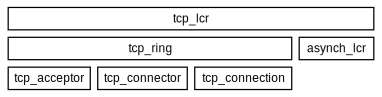
\includegraphics[width=\columnwidth]{tcp_lcr_automaton}
\caption{Architecture of the TCP LCR system.}
\label{tcp_lcr_automaton}
\end{figure}

The tcp\_lcr\_automaton which is listed in examples/tcp\_lcr.cpp\footnote{\url{github.com/jrwilson/ioa/blob/master/examples/tcp_lcr.cpp}} of the ioa++ package implements the complete protocol by composing an asynch\_lcr\_automaton and a tcp\_ring\_automaton.
Figure~\ref{tcp_lcr_automaton} shows the layered architecture of the TCP LCR system.
The bottom layer consists of component automata for TCP sockets, the middle layer consists of a component automaton that supports coordination via a unidirectional ring, and the top layer implements the business logic.
Thus, ioa++ supports features we expect from a component framework for distributed systems.

%% The key idea is that all of these modules have well-defined interactions when composed, while being inherently concurrent.
%% One need only focus on the protocol implemented by an automaton when composing it with an existing system, as opposed to worrying about interacting threads and race conditions.

\ifjournal
In this section, we explore whether ioa++ offers a suitably convenient representation for reifying I/O automata and contains the features necessary for building real distributed systems.
Our approach is to (1) express an automaton in ioa++ using an existing listing, (2) simulate a distributed system built using the automaton as debugging step, and (3) build a real distributed system by composing the automaton with automata for network services.
For continuity, we discuss further the asynchronous LCR automaton described in Section~\ref{programming_model}.

\paragraph*{Translating the asynchronous LCR automaton into ioa++}
The first version of the asynchronous LCR automaton was translated directly from a listing in~\cite{lynch1996distributed}, but was then refined with (1) an additional action to reinitialize the automaton and (2) modifications that allow an automaton that elected itself the leader to nullify its election.
The motivation for these modifications will be explained when we discuss its use in a real system.
The listing in~\cite{lynch1996distributed} consists of approximately 24 lines in a formal language that must be translated to a production language.
The raw listing for our final version consists of 121 lines (\~5x).
Scheduling accounts for 22 of the 121 lines (20\%) and is the main source of code that cannot be traced back to the formal listing.
On average, every local action contributed 6 lines of scheduling code and every input action contributed 3 lines of scheduling code.

We observe that having a representation of I/O automata in a production language (such as ioa++) which also closely matches a formal representation is of great benefit because it thus encourages one to reason about an automaton directly from the source code.
For example, an invariant in the asynchronous LCR automaton is that all of the UIDs in the send queue of automaton $i$ must be greater than or equal to the UID of automaton $i$.
This invariant can be quickly checked against the constructor and four actions of the asynch\_lcr\_automaton.
Upon construction, the send queue contains the UID of the automaton so the invariant holds initially.
The leader action does not modify the send queue so the invariant holds trivially.
The init action adds the automaton's UID to the send queue.
The receive action only adds a UID to the send queue if the UID is greater than the automaton's UID.
The send action removes a UID from the send queue.
Reasoning about an automaton directly from the source code allows one to use formal methods to develop and debug systems \emph{at the point of implementation directly}.

\paragraph*{Unit testing with simulation}
After the asynchronous LCR automaton was implemented, we developed a simulation to test it.
The examples/asynch\_lcr.cpp\footnote{Access directly at \url{http://github.com/jrwilson/ioa/blob/master/examples/asynch_lcr.cpp}.} file in ioa++ package contains the driver for the simulation.
The simulation creates a unidirectional ring of a specified size consisting of alternating asynch\_lcr\_automaton and channel\_automaton.
The channel\_automaton was also a direct translation from~\cite{lynch1996distributed}.

The simulation showed that the initial asynch\_lcr\_automaton was not correct.
The first bug we encountered was a silent failure where the ring failed to elect a leader.
The problem was that the leader action was never being scheduled, and to fix this the leader action was added to the scheduling function.
The second bug manifested itself by electing the wrong leader, i.e., one whose UID was not the maximum.
A closer inspection showed that certain UIDs were being sent but never received.
The key insight into solving the problem was to understand that the automata were executing as the ring was being constructed, i.e., we had failed originally to consider dynamic composition.
The solution was to add binding predicates to the outputs of the asynch\_lcr\_automaton and channel\_automaton.

\paragraph*{From abstraction to real system}
The next phase was to use the asynchronous LCR automaton to perform leader election in a real unidirectional ring of processes connected by TCP sockets.
The leader of the ring periodically sends a token which is forwarded by all nodes in the ring.
If a node has not received a token for a specified duration of time, it calls for an election.
This is the motivation behind the action that resets the asynch\_lcr\_automaton.
Nodes listen for connections from their predecessor and attempt to connect to their successor.
Nodes can join and leave the ring at any time.
The protocol should eventually succeed for complete rings and restart when a ring becomes incomplete.
These dynamics admit fault situations where a ring might lose its leader or contain multiple leaders.
A ring containing multiple leaders should stabilize to having a single leader.
This is the motivation behind the asynch\_lcr\_automaton being able to withdraw its election.
A rare (but possible and valid) situation is a ring circulating a token without a leader, i.e., the leader sends a token, leaves the ring, and is replaced before the token makes a full cycle.
This situation requires no action as a token is circulating in the ring.

The tcp\_lcr\_automaton which is listed in examples/tcp\_lcr.cpp\footnote{Access directly at \url{http://github.com/jrwilson/ioa/blob/master/examples/tcp_lcr.cpp}.} (484 lines) of the ioa++ package implements the protocol just described.
The tcp\_lcr\_automaton is a composition of a number of automata including an asynch\_lcr\_automaton, an ioa::tcp\_acceptor\_automaton, an ioa::tcp\_connector\_automaton, and two ioa::tcp\_connection\_automaton representing the channel from the predecessor and channel to the successor.
The TCP automata provided by the ioa++ package are ordinary automata implemented using file descriptors and the techniques described in Section~\ref{design}.
The tcp\_lcr\_automaton uses the techniques for managing dynamic constellations described in Section~\ref{programming_model}.

The tcp\_lcr\_automaton case study confirms that I/O automata can be a good foundation for building reusable concurrent modules.
The key idea is that all of these modules have well-defined interactions when composed, while being inherently concurrent.
For example, one could substitute the asynch\_lcr\_automaton with a different automaton to realize a different leader election protocol or a different protocol altogether.
Alternatively, the tcp\_lcr\_automaton could be refactored to use a different communication mechanism, e.g., UDP.
One need only focus on the protocol implemented by an automaton when composing it with an existing system, as opposed to worrying about interacting threads and race conditions.
\fi

%% Conclude with our recommendations for programming, highlight need for exploration.

%% Tips for Writing Programs with I/O Automata
%% 1. Make sure that a parameter exists.
%% 2. Move logic in observe to local actions.
%% 3. Avoid observing an arbitrary number of managers.
%% 4. Do not bind to managers allocated on the stack.
%% 5. Stop when an error is encoutered and report it.
%% 6. Make sure output actions are bound.
%% 7. Make sure local actions are scheduled.
%% 8. Do not pass pointers---use const_shared_ptr.
%% 9. Check preconditions.
%% 10. Check effects.
%% 11. Order clauses of preconditions for efficiency.
%% 12. Automata that should be destroyed at the same time should be created at the same time and vice versa.  (Group using a parent.)

%% \begin{outline}
%% \item State
%%   \begin{outline}
%%   \item There is no shared state in a 
%%   \item Local state only
%%   \item Shared state
%%     \begin{outline}
%%       \item Impossible in distributed systems
%%       \item Dangerous in local systems
%%     \end{outline}
%%   \end{outline}
%% \item Communication
%%   \begin{outline}
%%   \item Atomic asynchronous message passing
%%   \item Network sets size of atom (UDP)
%%   \item Can build reliable streams (TCP)
%%   \item Local equivalent is passing a value
%%   \item Model should lend itself to writing protocols
%%   \end{outline}
%% \item Asynchrony
%%   \begin{outline}
%%     \item Model must have natural support for asynchrony, i.e., event-based
%%     \item Leads to a more efficient implementation because changed state and enabled actions become obvious
%%   \end{outline}
%% \item Concurrency
%%   \begin{outline}
%%     \item Reason about systems using non-deterministic interleaving of atomic actions
%%     \item Model should admit implementations that execute concurrently
%%   \end{outline}
%% \item Dynamics
%%   \begin{outline}
%%     \item Configuration - Edges in graph of communicating components can change at run-time.
%%       \begin{outline}
%%       \item Already required in distributed settings
%%       \item Not addressed in formal models
%%       \end{outline}
%%     \item Extension - Nodes in graph of communicating components can change at run-time.
%%   \end{outline}
%%   \item Reflection
%% \end{outline}

%% I/O Automata
%% \begin{itemize}
%%   \item Compare with UNITY
%%   \item Compare with esterel
%%   \item Compare with pi calculus
%%   \item Compare with Ptolemy
%% \end{itemize}
